\section{Código fuente del web scraper}
El web scraper que ha rastreado internet para extraer la información de los lugares de interés ha sido programado en Python utilizando la librería Selenium.

Su código fuente es un script sencillo con el que se simula que un usuario está navegando por internet con el navegador de Google Chrome. Pero, básicamente, este ha buscado en Google Maps y ha recolectado la siguiente información de cada lugar:

\begin{itemize}
    \item Nombre.
    \item URL de la foto.
    \item Dirección.
    \item Coordenadas geográficas.
\end{itemize}

Toda la información recolectada la ha almacenado en un fichero de texto plano separado por carpetas llamadas igual que las categorías que se han establecido.

Además, he programado otro script, en Python, que realiza las siguientes operaciones:
\begin{itemize}
    \item Descarta los sitios que tengan el mismo nombre dentro de la misma categoría, ya que presumiblemente serán el mismo lugar.
    \item A cada lugar le asigna la zona de la isla, de las que se han definido dentro de la aplicación, que le corresponda por sus coordenadas geográficas. Las divisiones en zonas de la isla será definida en su propia sección dentro del quinto capítulo.
    \item Genera un fichero en formato JSON con los sitios que aparecen en más de una categoría. Estos deben ser revisados manualmente.
    \item Genera un fichero en formato JSON con el resto de sitios, dividiéndolos por categoría.
\end{itemize}

\section{Estructura código fuente de la aplicación}
Para el desarrollo del código fuente de la aplicación se ha seguido el paradigma de programación orientado a objetos y también se ha hecho uso de eventos, ya que este es el modelo con el que trabaja Unity. Además, para cada pantalla se han utilizado diferentes escenas, las cuales serán explicadas a continuación.

\subsection{Escenas}
Los proyectos de Unity son, comúnmente, divididos en escenas. Para desarrollar DiscoverTenerife se ha seguido ese patrón de escenas independientes con algunos objetos que permanecen entre escenas para conservar información, como es el caso de firebaseHandler o gpsController. 

Las escenas en las que se ha dividido el proyecto coinciden con las diferentes pantallas que nos encontramos en la aplicación:

\begin{itemize}
\item \textbf{Login}: Pantalla sencilla con 5 botones que dirigen a los diferentes métodos de inicio de sesión o de registro. Tenemos las siguientes opciones que nos dirigen a otras pantallas: 
\begin{itemize}
    \item \textbf{Sign In}: Para iniciar sesión mediante correo y contraseña, debemos tener una cuenta previamente creada.
    
    \item \textbf{Register}: Para registrarse como nuevo usuario mediante correo y contraseña.
    
    \item \textbf{Iniciar sesión con Google}: Para iniciar sesión utilizando la autenticación de Google, debemos tener una cuenta previamente creada con Google para acceder de esta forma.
    
    \item \textbf{Registrarse con Google}: Para crear una cuenta utilizando la autenticación de Google.
    
    \item \textbf{Inicio de sesión anónimo}: Para iniciar sesión utilizando la de usuario anónimo de firebase. Este sistema ha sido incluido para usuarios que solo quieran utilizar la aplicación como una guía turística convencional, sin utilizar factores competitivos o sociales. Este tipo de cuentas no están recomendadas porque están ligadas al dispositivo, es decir, si se cambia de dispositivo, se desinstala la aplicación o se borran los datos de la aplicación, se perderá todo el progreso dentro de la aplicación.
\end{itemize}

\item \textbf{Principal}: En esta pantalla encontramos diferentes elementos, un botón que nos llevará a la sección de ajustes, un texto que nos indica en qué zona de la Isla estamos y dos barras de experiencia, una indica el porcentaje de lugares visitados dentro de la zona actual y el otro indica el porcentaje de lugares visitados de todo Tenerife.

Además, se nos mostrarán una serie de lugares en un panel que es deslizable, si deslizamos hacia arriba lo suficiente recargaremos la escena consiguiendo que actualice la lista de lugares teniendo en cuenta nuestra ubicación actual. 

En cambio, si deslizamos hacia abajo, se irán mostrando nuevos lugares ordenados según las preferencias que se hayan definido en la pantalla de ajustes, las cuales serán explicadas más adelante. Se mostrarán hasta 15 lugares, si seguimos deslizando hacia abajo, hasta cierto punto, conseguiremos que la escena recargue teniendo en cuenta que ya hemos visto esos 15 lugares, por lo tanto, tras la recarga se nos mostrarán los siguientes 15 puntos de interés ordenados de nuevo por los ajustes que hayamos decidido.

Si pinchamos sobre alguno de los lugares que se nos ofrecen accederemos a la pantalla de ese lugar, esta pantalla será explicada a continuación.

\begin{figure}[H]
    \centering
    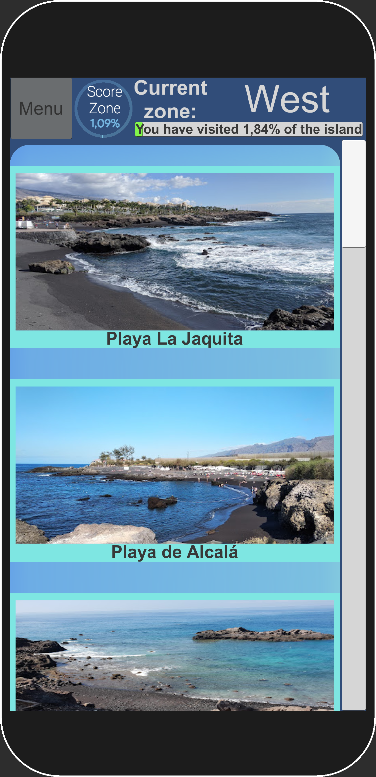
\includegraphics[width=0.25\textwidth]{Memoria_TFG_LaTeX/images/pantallaPrincipal.PNG}
    \caption{Demostración de cómo es la pantalla principal.}
    \label{fig:pantallaPrincipal}
\end{figure}

\item \textbf{Lugar}: En esta pantalla se nos presentará toda la información relativa al lugar: 
    \begin{itemize}
    \item Un cartel que indica si lo hemos visitado previamente o no.
    
    \item Una foto.
    
    \item El nombre, la distancia al usuario, calculada accediendo al sistema de geolocalización del dispositivo del usuario y la dirección, si la dirección no estuviera disponible, se presentarían las coordenadas geográficas exactas de ese punto de interés.
    
    \item Una barra que cambia de color de verde a rojo y de relleno de izquierda a derecha en función de la cantidad de visitas que tenga ese lugar comparado con el resto de lugares.
    
    \item Por último, encontramos 4 botones:
        \begin{itemize}
            \item \textbf{Google Maps}: Abre la aplicación de Google Maps con las coordenadas del punto de interés marcadas en el mapa.
            
            \item \textbf{Retar a un amigo}: Abre una pantalla que nos muestra los amigos que tenemos y se da la opción de retarles a visitar este sitio, siempre y cuando, ese amigo no tenga ya un reto nuestro y haya pasado al menos 7 días desde el último reto que le hayamos enviado.
            
            \item \textbf{Guardar el lugar para una visita sin conexión a Internet}. Podremos guardar hasta 5 lugares para visitar sin conexión.
            
            \item \textbf{Registrar este lugar como visitado}: Si el usuario está suficientemente cerca, al menos a 50 km, y ha cumplido el tiempo de enfriamiento, de 1 hora de tiempo real, se registrará el lugar como visitado y el usuario ganará puntos.
        \end{itemize}
    \end{itemize}

\begin{figure}[H]
    \centering
    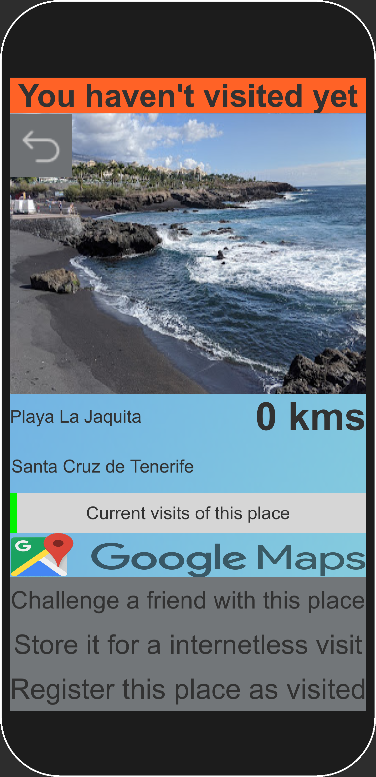
\includegraphics[width=0.25\textwidth]{Memoria_TFG_LaTeX/images/pantallaLugar.PNG}
    \caption{Demostración de cómo se ve la pantalla de un lugar cuando el usuario no lo ha visitado.}
    \label{fig:pantallaLugarNoVisitado}
\end{figure}

\begin{figure}[H]
    \centering
    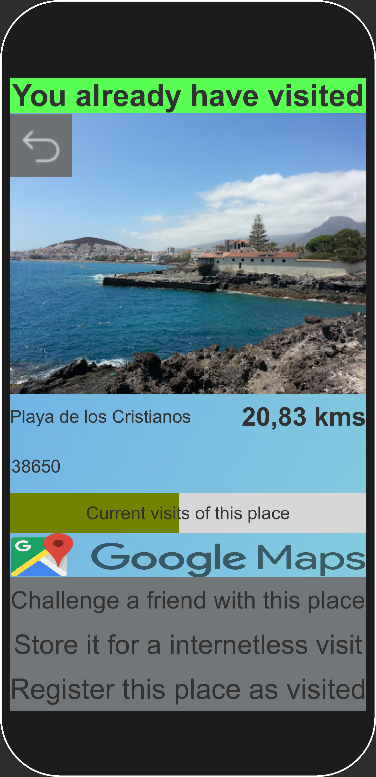
\includegraphics[width=0.25\textwidth]{Memoria_TFG_LaTeX/images/pantallaLugarVisitado.PNG}
    \caption{Demostración de cómo se ve la pantalla de un lugar cuando el usuario lo ha visitado.}
    \label{fig:pantallaLugarVisitado}
\end{figure}

\item \textbf{Menú}: En esta escena se nos muestran una serie de botones que nos llevan a otras pantallas que nos permiten hacer lo que su nombre indica. Las opciones disponibles son:

\begin{itemize}
    
    \item \textbf{Historial de sitios visitados}: pantalla que muestra la lista de lugares que ha visitado el usuario.
    
    \item \textbf{Ranking de jugadores}: pantalla que muestra la lista de jugadores que permiten aparecer en el ranking ordenado por puntuación.
    
    \begin{figure}[H]
    \centering
    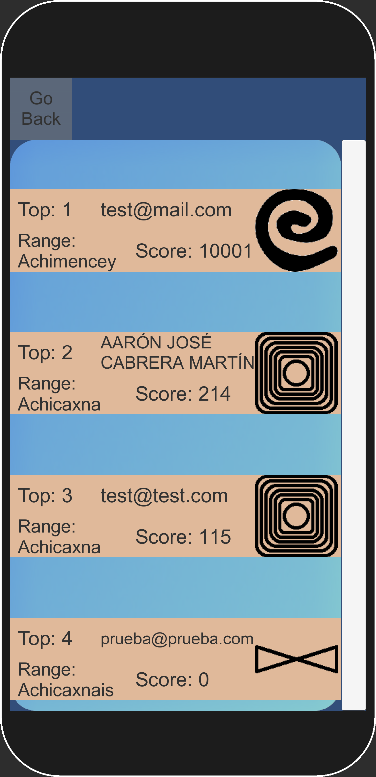
\includegraphics[width=0.25\textwidth]{Memoria_TFG_LaTeX/images/pantallaRanking.PNG}
    \caption{Demostración de cómo se ve la pantalla del ránking.}
    \label{fig:pantallaRanking}
    \end{figure}
    
    \item \textbf{Mi rango y puntuación}: pantalla que muestra nuestro rango, con su respectivo icono y puntuación actual. También se muestra la fecha en la que hemos ascendido a los anteriores rangos.
    
    \item \textbf{Mis estadísticas}: pantalla que muestra el porcentaje de lugares visitados de cada zona de la Isla por separado que llevamos. También se nos muestra la cantidad de lugares diferentes que hemos visitado, la cantidad de visitas acumuladas y el lugar, la zona y el tipo de lugar que más hemos visitado.
    
    \item \textbf{Mis amigos}: pantalla que muestra la lista de amigos que tenemos. Desde aquí podemos retar a un amigo a visitar algún lugar que hayamos guardado anteriormente o eliminar a ese amigo.
    
    \item \textbf{Nuevas invitaciones a amigo}: pantalla que muestra una lista de solicitudes de amistad. Desde esta pantalla podemos, eliminar esa invitación o aceptarla.
    
    \item \textbf{Buscar un nuevo amigo}: pantalla que nos muestra una barra de búsqueda. Si escribimos en ella, se nos mostrarán aquellos jugadores que en su nombre contengan la cadena que hemos escrito y que hayan permitido que otros jugadores les envíen invitaciones de amistad.
    
    \item \textbf{Lugares guardados para una visita sin internet}: en esta pantalla se nos muestra la lista de lugares que tenemos guardado para visitar cuando no tengamos conexión a internet, podemos intentar visitar ese lugar o eliminarlo. Cabe recordar, que para visitar el sitio, seguiremos necesitando la geolocalización. Las visitas que realizamos de esta manera serán subidas al servidor desde que tengamos conexión a internet.
    
    \begin{figure}[H]
    \centering
    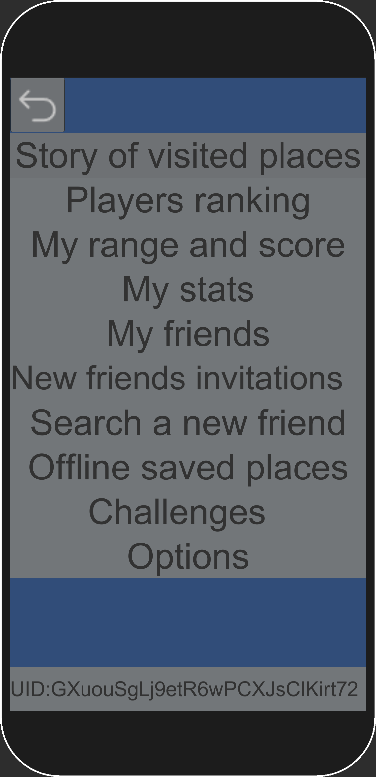
\includegraphics[width=0.25\textwidth]{Memoria_TFG_LaTeX/images/pantallaMenu.PNG}
    \caption{Demostración de cómo se ve la pantalla del menú.}
    \label{fig:pantallaMenu}
    \end{figure}
    
    \item Opciones: en esta sección podremos configurar:
    \begin{itemize}
        \item \textbf{Unidad de medida de la distancia}: kilómetros o millas.
        
        \item \textbf{Tipos de lugares} que queremos encontrar o si deseamos ver lugares ya visitados. Si marcamos que no queremos ver lugares ya visitados, estos tendrán la prioridad mínima al elegir los lugares que se muestran en la pantalla principal.
        
        \item \textbf{Reglas para ordenar los lugares}: si, por menor distancia a tu ubicación o por menor número de visitas del lugar.
        
        \item \textbf{Opciones sociales}: En este apartado podremos elegir si deseamos aparecer en el ranking de usuarios, si deseamos permitir que otros usuarios nos envíen peticiones de amistad y si deseamos permitir que otros amigos nos envíen retos.
        
        \item \textbf{Cerrar sesión}: Con este botón podremos cerrar sesión y volver a la pantalla de inicio de sesión o creación de cuenta.
        
        \item \textbf{Reportar un error}: Si pulsamos este botón se nos abrirá la aplicación de correo electrónico por defecto, por ejemplo, Gmail con un correo preparado, con un texto indicando al usuario que describa lo que ha ocurrido y avisándole de que si puede añadir una captura de pantalla el reporte será mucho más útil.
        
    \end{itemize}
\end{itemize}


\end{itemize}

\subsection{Clases Principales}
\begin{itemize}
\item \textbf{firebaseHandler}: Se encarga de manejar todos los eventos o funciones relacionadas con la base de datos Firebase, el backend de la aplicación. Esta clase ha sido divida en varios ficheros con clases parciales para facilitar su lectura.
Las clases parciales que he realizado han sido:
\begin{itemize}
    \item \textbf{firebaseHandler}: Se trata de la parte principal, se encarga de controlar cuando se puede subir o descargar la información desde el servidor, teniendo en cuenta el estado actual de la conexión a internet. Si no hay conexión a internet, genera una serie de colas que almacenan qué cambios se deben subir para que, desde que se consiga una conexión estable, se suba toda esa información.
    
    \item \textbf{loginHandler}: Encargado de todo el sistema de login de usuarios y registro de nuevos usuarios.
    
    \item \textbf{downloadHandler}: Contiene todos los métodos que descargan información del servidor.
    
    \item \textbf{uploadHandler}: Contiene todos los métodos que suben información al servidor.
    
\end{itemize}

Es decir, el conjunto de ficheros que forman la clase firebaseHandler contiene métodos para crear nuevos usuarios o para iniciar sesión con cada uno de los métodos permitidos. Además, almacena la información del usuario cuando este inicia sesión, la información relativa al usuario es almacenada con un objeto de la clase \textbf{UserData}. La instancia de esta clase es única por cada ejecución y permanece entre escenas. FirebaseHandler también contiene una instancia de la clase \textbf{requestHandler} la cual almacena toda la información relativa a los lugares de interés y lleva el control del orden en el que el usuario debe acceder o visualizar estos, teniendo en cuenta las opciones que el usuario ha seleccionado en la correspondiente pantalla.

\item \textbf{UserData}: Es la encargada de almacenar toda la información relativa al usuario una vez ha iniciado sesión. Se almacena el identificador de usuario, los sitios que ha visitado y el nombre que posee.

\item \textbf{Place}: Se encarga de almacenar la información relativa a un punto de interés, por lo tanto, en tiempo de ejecución existirán varias instancias de esta clase. Posee un método para realizar la descarga de la imagen a través de internet.

\item \textbf{gpsController}: Se encarga de gestionar el acceso al sistema GPS del dispositivo. Además, tiene métodos para verificar que los permisos de acceso al sistema GPS han sido concedidos. La instancia de esta clase permanecerá entre la pantalla principal y la pantalla de un lugar concreto.

\item \textbf{optionsController}: Se encarga de almacenar la configuración actual que el usuario ha escogido, también refleja esos cambios en la pantalla de opciones. La instancia de esta clase permanecerá entre la pantalla principal, la pantalla de un lugar concreto, la pantalla de opciones y la pantalla de estadísticas del usuario.

\item \textbf{MapRulesHandler}: Esta clase contiene atributos y métodos únicamente estáticos. No está pensada para ser instanciada, se comporta como un almacén para la información que únicamente variará si se cambia la zona del planeta en la que trabaja la aplicación.

\item \textbf{gameRules}: Esta clase contiene atributos y métodos únicamente estáticos. No está pensada para ser instanciada, se comporta como un almacén de información o funciones relativas a las reglas del juego. Almacena, por ejemplo, cuánto tiempo tiene que pasar entre dos visitas consecutivas a un lugar o las fórmulas que calculan la puntuación que obtiene el usuario al visitar un lugar o al completar un reto, etc.
\end{itemize}

Recordar que la documentación del código fuente se encuentra disponible en el Github Pages del proyecto\cite{doxygenDiscoverTenerife} y que puede ser consultada para obtener unas mejores explicaciones de como funciona el código interno de la aplicación, ya que allí, se encuentra esta información más extensamente explicada.


\section{Estructuración de la base de datos}

Tras varias iteraciones, se ha decidido dividir la base de datos en dos sectores principales, los lugares y la información de los usuarios. Finalmente, el diseño que se ha llevado a cabo para implementar ha sido el que se presenta a continuación:

\begin{itemize}
\item \textbf{Lugares}: Tiene una entrada por cada tipo de punto de interés: \textbf{Playas}, \textbf{miradores}, \textbf{rutas de senderismo}, \textbf{parques naturales} y \textbf{piscinas naturales}. A su vez, cada una de estas categorías almacena, utilizando un identificador numérico, la información de cada punto de interés. Por lo tanto, la clave primaria de cada punto de interés sería la tupla: tipo de sitio de interés e identificador numérico.

La información almacenada de cada punto de interés es:
\begin{itemize}
    \item \textbf{Dirección}, si el sitio no posee dirección, se rellena el campo con las coordenadas geográficas.
    \item \textbf{Link a la imagen} del lugar, para la futura descarga de la imagen.
    \item \textbf{Latitud} del punto geográfico donde se encuentre el punto de interés.
    \item \textbf{Longitud} del punto geográfico donde se encuentre el punto de interés.
    \item \textbf{Nombre} del lugar.
    \item \textbf{Número de veces} que ha sido visitado.
    \item \textbf{Zona} de Tenerife en la que se encuentra.
\end{itemize}

\item \textbf{Usuarios}: Almacena una entrada por cada usuario. Donde la clave es el UID\footnote{\textbf{UID}: Siglas de User ID, ID es la abreviación de la palabra Identification. Traducido al español significa: Identificador de Usuario} del propio usuario. Se almacena la siguiente información de cada usuario:
    \begin{itemize}
    \item \textbf{Display name}: nombre del usuario.
    \item \textbf{Places Visited}: Lista ordenada cronológicamente por la \textbf{primera} visita que ha realizado dicho usuario a ese lugar. La clave es un identificador numérico que indica el orden cronológico de la primera visita. Por cada entrada de la lista se almacenan los siguientes valores:
        \begin{itemize}
        \item Identificador numérico del lugar.
        \item El tipo del lugar.
        \item Última vez que ese usuario ha visitado ese lugar, para controlar el tiempo de espera entre visita y visita.
        \item Cuántas veces ha visitado ese usuario ese punto.
        \end{itemize}
    \item \textbf{Base Coords}: Coordenadas del lugar en el que el usuario realizó la primera conexión. Estas coordenadas quedan registradas para poder calcular puntuación extra obtenida por visitar lugares que están más lejos de la zona que presumiblemente suele frecuentar.
    
    \item \textbf{Challenges}: Lista que almacena los retos que tiene el usuario. Cada reto almacena: el usuario que envió el reto, el timestamp del momento en el que el reto fue enviado y la información necesaria para diferenciar el lugar; tipo e id.
    
    \item \textbf{EarnedScore}: Entero que almacena la puntuación que el usuario ha conseguido de forma pasiva. En el prototipo actual, la única forma de conseguirla es cuando un amigo completa uno de nuestros retos.
    
    \item \textbf{Friends}: Lista que contiene los uids de aquellos jugadores a los que hemos aceptado como amigo o los cuales nos han aceptado como amigos.
    
    \item \textbf{RangeStory}: Lista que almacena un elemento cada vez que el usuario sube de rango. Se almacena el rango alcanzado y la fecha.
    
    \item \textbf{Score}: Entero que almacena la puntuación actual del usuario.

    \item \textbf{FriendInvitations}: Lista que almacena las peticiones de amistad que nos han enviado otros usuarios y que aún no hemos respondido.
    
    \item \textbf{AcceptedFriendInvitations}: Lista de las peticiones de amistad que hemos enviado y que el usuario destino ha aceptado. Esta lista se vacía cada vez que el usuario se conecta, los user id que aparecen en esta lista son movidos a la lista de Friends.
    
    \item \textbf{DeletedFriends}: Lista de uids de usuarios que eran nuestros amigos, pero que han decidido eliminar la amistad. Esta lista se vaciará en cada login. Todos los user id que se encuentren en esta lista serán eliminados de la lista Friends sin notificar nada al usuario.
    
    \end{itemize}

\item Usuarios que permiten recibir \textbf{peticiones de amistad}: Lista de uids de los usuarios que tienen habilitada la opción de recibir peticiones de amistad de otros usuarios. Si tienen desactivada esa opción, son eliminados de esta lista y, por lo tanto, la única manera que tienen de establecer una amistad es ellos mismos mandar la invitación a otro usuario que sí tenga esa opción activada.

\item Usuarios que permiten aparecer en el \textbf{ránking de usuarios}: Lista de uids de usuarios que tienen habilitada la opción de aparecer en el ránking de usuarios. Si tienen desactivada esta opción, no se les tendrá en cuenta a la hora de calcular las posiciones del ránking de usuarios.

\item Usuarios que permiten \textbf{ser retados por otros usuarios}: Lista de uids de usuarios que tienen activada la opción de que sus amigos les envíen retos. Si tienen esta opción desactivada, cuando alguno de sus amigos intente retarles, directamente no les aparecerá en la lista de usuarios rentables.

\end{itemize}

\subsection{Reglas de seguridad de la base de datos}
Una vez establecida la estructura de la base de datos, el siguiente paso ha sido establecer unas reglas de seguridad apropiadas. Las reglas que se han establecido son:
\begin{itemize}
\item Cualquier petición de un usuario no identificado se rechaza.
\item Todos los usuarios autentificados pueden leer la información de los sitios de interés.
\item Todos los usuarios autentificados pueden sobreescribir el valor de la propiedad ``número de veces visitado`` de todos los sitios de interés.
\item En la parte de usuarios, los usuarios únicamente pueden leer y escribir la información de su propia entrada, excepto las listas de ``acceptedFriends``, ``deletedFriends``, ``earnedScore`` y ``challenges``. Estas listas pueden ser modificadas por cualquier usuario identificado que además no sea anónimo. Esto es así para permitir establecer relaciones de amistad, eliminar relaciones de amistad, retar a otros jugadores u obtener puntuación por haber hecho que un amigo complete uno de tus retos. Se excluye a los jugadores anónimos del permiso de escritura de estas listas porque, estos jugadores no tienen permitido el acceso a las funcionalidades sociales que utilizan estas características. 

\end{itemize}
Con estas reglas, se les permite a los usuarios autentificados leer toda la información de los sitios de interés, pero solamente escribir el único campo que depende de ellos; el número de veces visitado. Y se impide que los usuarios puedan escribir en los campos de otros usuarios, excepto los que son necesarios.

También es importante destacar que en las listas; ``usersThatAllowFriendshipsInvitations``, ``usersThatAllowBeChallenged``, ``usersThatAllowAppearedOnRanking``, en las cuales están apuntados los id de usuario de cada usuario que permite; recibir invitaciones de amistad, ser retado por sus amigos o aparecer en el ránking respectivamente. Cada usuario puede elegir si estar o no en cada una de esas listas en el menú de opciones, por lo tanto, todos los usuarios autentificados pueden añadir o eliminar su uid de cualquiera de las tres listas.

\subsection{Métodos de autenticación}
La gestión de usuarios es otra herramienta que ofrece Firebase, para este proyecto se ha decidido utilizar los siguientes métodos de autentificación:
\begin{itemize}
\item \textbf{Correo electrónico y contraseña}: Introduciendo un correo electrónico y una contraseña de, al menos, seis dígitos de longitud, un usuario puede registrarse e iniciar sesión.
\item \textbf{Inicio de sesión con Google}: Utiliza una sesión iniciada previamente de una cuenta Google del dispositivo, es la opción más segura y recomendada.
\item \textbf{Inicio de sesión anónimo}: Este método que incluye firebase consiste en generar un User ID para esa instancia de ese dispositivo, es decir, si se borra los datos de la aplicación, se desinstala la aplicación y luego se instala de nuevo o si se cambia de terminal móvil, se perderá la información del usuario. Este método, puesto que fácilmente se puede perder el progreso conseguido, sólo está recomendado para un primer contacto con la app, o para los usuarios que quieran utilizar la aplicación solamente para descubrir los lugares, como si se tratase de una guía turística tradicional.
\end{itemize}